\section{Outlier detection}

\begin{figure}
    \centering
    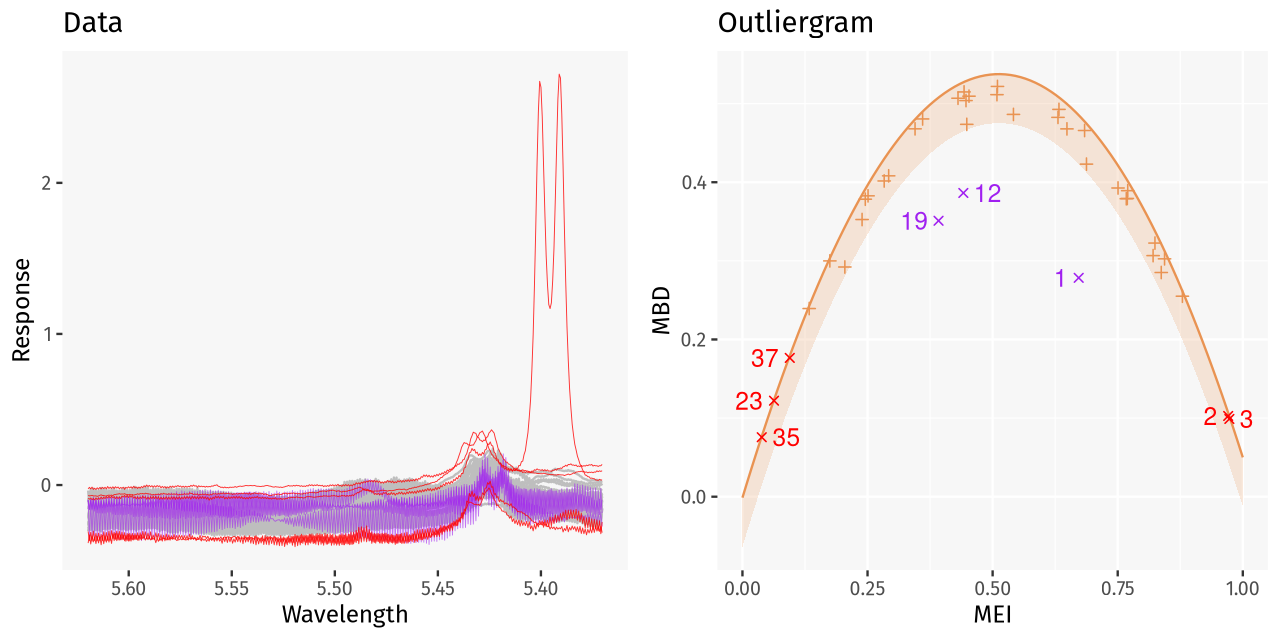
\includegraphics[width = \textwidth]{outliergram_wine}
    \caption{
        Outliergram for the NMR spectra of 40 wine samples.
        The three purple curves have been identified as shape outliers, as
        they fall outside the orange ribbon in the outliergram.
        Although the red curves lie on the orange parabola, they have low MBD
        and extreme MEI values, indicating that they lie above or below the
        main mass of curves.
    }
    \label{fig:outliergram_wine}
\end{figure}



\begin{figure}
    \centering
    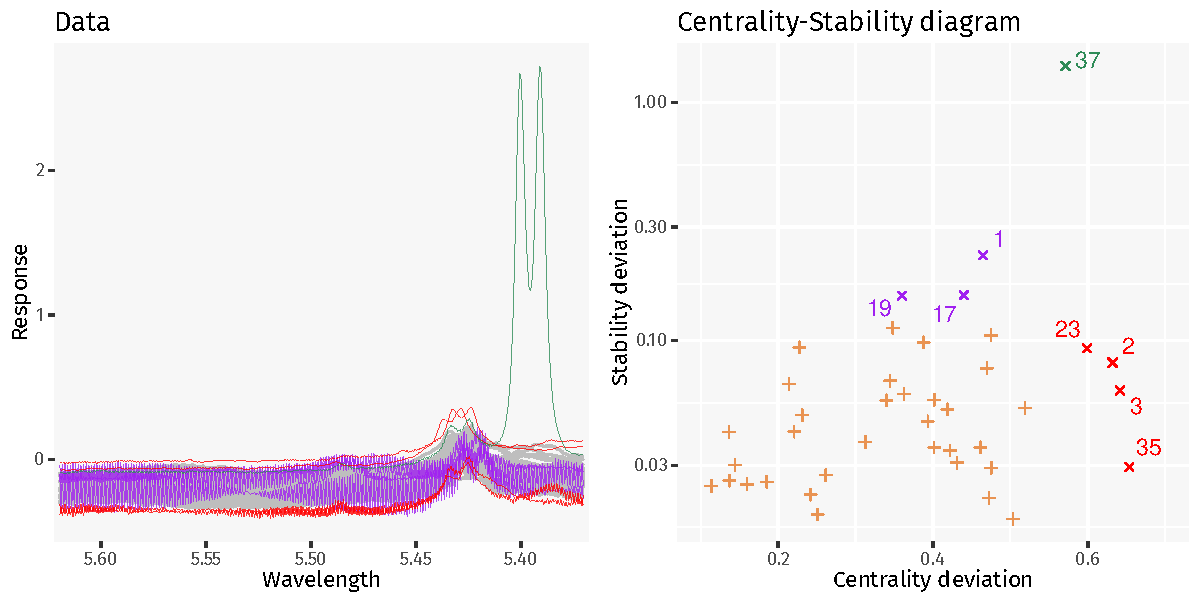
\includegraphics[width = \textwidth]{centrality_stability_wine}
    \caption{
        Centrality-stability diagram for the NMR spectra of 40 wine samples.
        The red curves are seen to deviate in terms of centrality, indicated
        by the fact that the corresponding points in the centrality-stability
        diagram fall towards the right.
        The purple curves deviate in terms of stability, with the green curve
        showing extreme deviation.
    }
    \label{fig:centrality_stability_wine}
\end{figure}


\begin{figure}
    \centering
    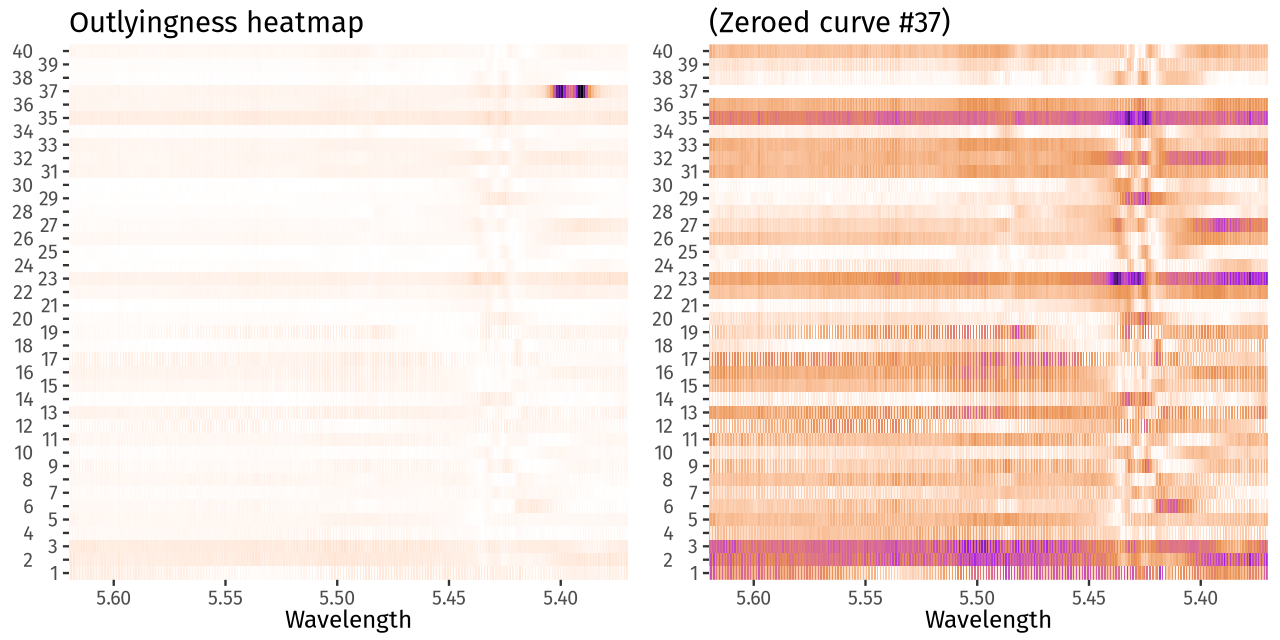
\includegraphics[width = \textwidth]{outlyingness_heatmap_wine}
    \caption{
        Outlyingness heatmap for the NMR spectra of 40 wine samples.
        The extreme curve #37 has been zeroed out in the second diagram to
        better illustrate the variation in outlyingness for the remaining
        curves.
    }
    \label{fig:outlyingness_heatmap_wine}
\end{figure}



\begin{figure}
    \centering
    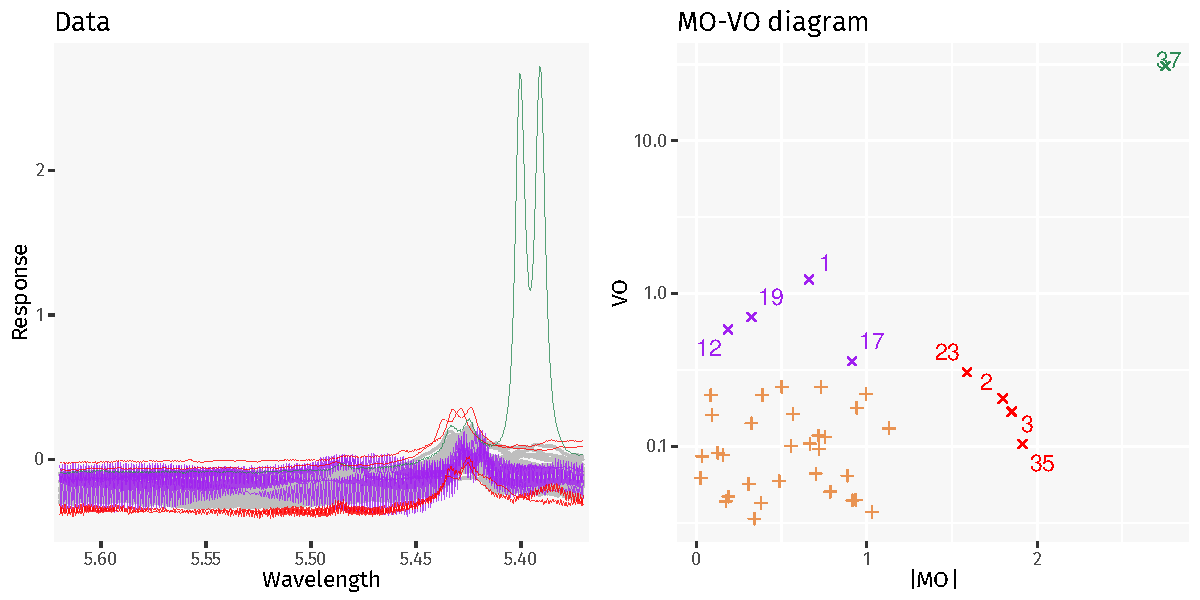
\includegraphics[width = \textwidth]{MO_VO_wine}
    \caption{
        MO-VO diagram for the NMR spectra of 40 wine samples.
    }
    \label{fig:MO_VO_wine}
\end{figure}



